\section{Introduction}

%%Here is a problem
%Upcoming memory technologies, such as Intel's recently-announced XPoint-3D
%memory, are projected to be denser and cheaper per bit than DRAM while providing
%the byte-addressable load-store interface of conventional main memory.  Improved
%capacity and cost per bit comes at the price of higher access latency, projected
%to fall somewhere in the range of 500ns to several microseconds~\cite{xpoint}.
%The impending commercial availability of such devices has renewed interest in
%two-tiered physical memory, wherein part of a system's physical address space is
%implemented with the slower, cheaper memory technology.  Slow memory can result
%in a net TCO win if the cost savings of replaced DRAM outweigh cost increase due
%to reduced program performance or by enabling a higher peak memory capacity per
%server than is economically viable with DRAM alone.  Our preliminary results
%indicate that over half of the memory footprint of representative cloud
%applications (e.g., Cassandra) are identified as cold by Linux’s kstaled
%mechanism, indicating that the corresponding pages have an inter-access interval
%exceeding 120s.  Analytic modeling suggests these pages could be shifted to a
%memory with a 3us access time with negligible (<3\%) performance degradation.
%
%%It's an interesting problem
%Prior academic work has considered two approaches to two-tiered memory: via a
%paging mechanism~\cite{Ekman2005,Lim2009}, wherein accesses to slow memory
%invoke a page fault that must transfer data to fast memory before an access may
%proceed, and via a migration mechanism (as in cache coherent NUMA
%multiprocessors)~\cite{Lim2009}, wherein no software fault is required.  In the
%latter scenario, a migration mechanism seeks to shuffle pages between tiers to
%maximize fast-memory accesses.  
%
%%It's an unsolved problem
%However, all prior work on two-tiered memory has assumed migration/paging at 4KB
%page granularity.  Huge pages, implemented via Linux's Transparent Huge Page
%(THP) mechanism, are now ubiquitous and critical for cloud applications.
%Recent work~\cite{JeffPaper} has demonstrated that 2MB huge pages are particularly
%performance-critical under virtualization.  For example, our study demonstrates
%a 20\% throughput improvement for Hadoop and a 40\% speedup on random memory
%probes when using huge pages under virtualization.  Huge pages thwart prior
%two-tiered memory proposals for two reasons: (1) it is too expensive to
%frequently migrate pages at 2MB granularity, and (2) hot regions occur within
%otherwise cold 2MB huge pages. 
%
\begin{figure}[t]
\centering
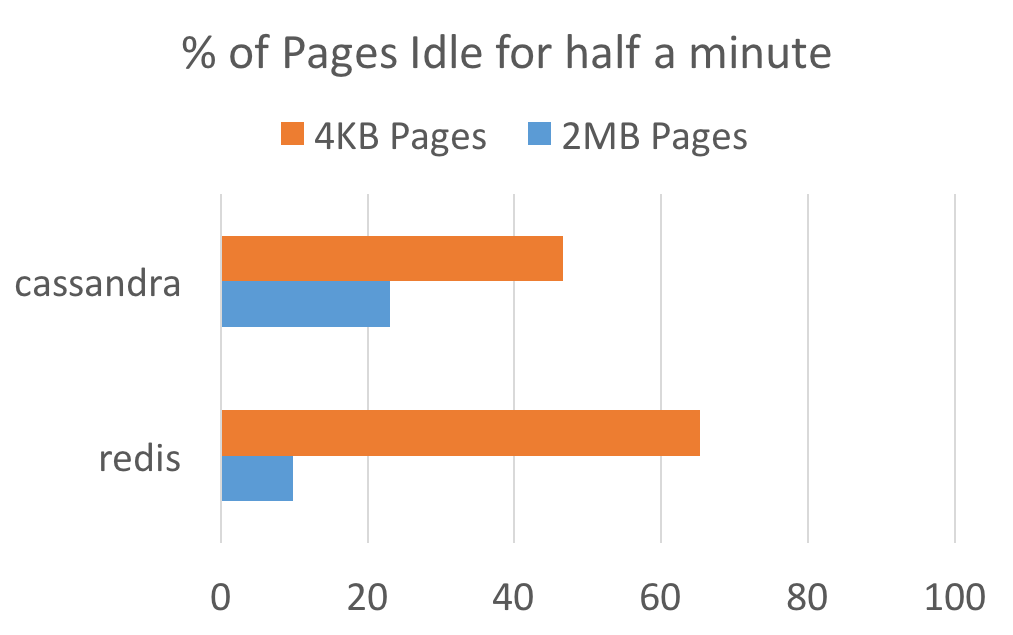
\includegraphics[width=1.0\columnwidth]{thermostat/figures/cold-data.png}
\caption{Amount of cold data in applications, thp vs no-thp numbers}
\vspace{-0.175in}
\label{fig:motivation-thermostat}
\end{figure}

%%Here is my idea
%Our Proposal: We propose to develop a transparent huge-page-aware two-tiered
%memory solution that integrates support for dynamic page migration and
%transparene huge pages, achieving both the capacity/cost advantages of
%two-tiered memory and performance advantages of huge pages.  Our focus is on
%cloud computing scenarios where a high-memory-footprint application, such as
%Cassandra, Aerospike, or MySQL, runs under virtualization and may co-run with
%other, competing applications.
%
%Hot regions within otherwise cold huge pages present a central challenge to our
%objective; existing x86-Linux provides no mechanism to carve out a 4KB hot
%region within a 2MB cold page.  So, we propose translation facades, a 4KB
%translation that remaps a portion of a 2MB mapping with an alternate physical
%address or permissions.  Current x86-Linux requires non-overlapping mappings due
%to hard-coded page table structure and because TLB entries are replaced
%independently, hence, an uncached 4KB facade to a cached 2MB translation could
%lead to a mis-translation. We will pursue implementations of translation
%facades along two paths. (1) Hardware support: we will extend x86 page table and
%TLB design to support facades. (2) Virtualization: Our existing study of huge
%pages under virtualization demonstrate that a majority of the benefit can be
%obtained if host pages are 2MB even if guest pages are 4KB.  We will investigate
%if the two-level translation from guest to host to machine addresses can be
%exploited to emulate hardware support for translation facades.
%
%%Bulleted list of contributions
%Our research program will follow a four-fold approach.  (1) We will measure hot
%and cold memory fractions at 4KB granularity and within 2MB huge pages to
%measure two-tiered memory opportunity and demonstrate the need for translation
%facades. We will use kstaled (an optional extension to the Linux kernel that
%tracks pages that have not been accessed over a fixed time interval) and
%BadgerTrap [4] (a tool to intercept soft page faults) to facilitate this
%characterization. (2) We will develop methods to track hot and cold memory
%regions at run-time.  A key challenge lies in efficiently tracking hot regions
%within an otherwise-cold huge page, as kstaled provides visibility only at page
%granularity.  We propose to investigate sampling methods, e.g., by
%probabilistically demoting huge pages or leveraging performance counter
%infrastructure. (3) We will develop an online migration mechanism that can shift
%data between fast and slow memory tiers while the application is concurrently
%executing. We draw experience from existing NUMA migration and THP memory
%defragmentation. We will implement the migration mechanism in the Linux kernel.
%(4) We will develop translation facades (using BadgerTrap to emulate
%performance) and investigate novel page table and TLB organizations to support
%facades.

%TODO My idea works
%TODO Here's how my idea compares to other people's approaches

%OLD TEXT
%
Upcoming memory technologies such as Intel 3D-XPoint~\cite{xpoint} are an
attractive candidate for reducing main memory costs (both in terms of CapEx and
OpEx) in datacenters, which is pegged at 30\% of TCO by recent
estimates~\cite{XXX}. Such memory technologies have two defining characteristics
that set them apart from commodity DRAMs: a) they are much cheaper per unit
capacity than DRAM, with current estimates putting them at $50\%$ cheaper
than DRAM, and, b) they are much slower than DRAM technology. Whereas
commodity DDR3/DDR4 has a latency of $\approx$100ns, such upcoming memory
technologies have latencies of the order of 400ns--1us.

Because of such high access latencies of newer memory technologies, they can not
completely substitute DRAMs. Instead, a prime area for such technologies is for
storing {\it cold} data of applications.  Our preliminary results shown in
Figure~/ref{fig:motivation} indicate that over half of the memory footprint of
representative cloud applications (e.g., Cassandra) are identified as cold by
Linux’s kstaled mechanism, indicating that the corresponding pages have an
inter-access interval exceeding 120s.  Analytic modeling suggests these pages
could be shifted to a memory with a 3us access time with negligible (<3\%)
performance degradation.

%It has been shown
%that a major fraction (XXX\% by some estimates~\cite{XXX}) of application
%footprint in current cloud/datacenter workloads is {\it cold}, i.e., rarely
%touched by the application. 

Placing such data in slow memories does not degrade the application throughput
or latency significantly, while also reducing the amount of costly DRAM required
in datacenters by a significant margin. In order to perform such placement in a
application-transparent fashion, the identification of cold data is done at an
OS page granularity, where a page is deemed to be a ``hot page'' if any of the
data present in that page is hot.

As a consequence of this mechanism, when going to larger page sizes (2MB/1GB
instead of the currently prevailing 4KB), a significantly smaller fraction of
pages is classified as ``cold''. This is because the presence of even a {\it
single} hot data item in an otherwise cold page will result in the entire page
being classified as hot. Using a smaller page size could have identified the
locations of the hot data more precisely, and thereby resulted in a larger
fraction of cold pages. Such a ``hotspot'' distribution of hot data is common in
datacenter applications, and according to our estimates, using 2MB sized pages
reduces the fraction of cold pages by $\approx$2-3$\times$. Thus, using larger
page sizes cause sub-optimal usage of cheap memory technologies in datacenters.

However, usage of large page sizes, typically done in Linux through {\it
Transparent Huge Pages (THP)}, is ubiquitous in modern datacenter applications.
THP is a mechanism available in the Linux kernel whereby applications can
transparently use large (2MB) or huge (1GB) sized pages without any source code
change. Larger page sizes has been shown to reduce page faults and thereby
improve throughput and latency in datacenter applications significantly.  Recent
work~\cite{JeffPaper} has demonstrated that 2MB huge pages are particularly
performance-critical under virtualization.  For example, our study demonstrates
a 20\% throughput improvement for Hadoop and a 40\% speedup on random memory
probes when using huge pages under virtualization.  However, huge pages pose two
challenges to prior two-tiered memory proposal: (1) migrating pages at 2MB
granularity is expensive, and (2) hot regions occur within otherwise cold 2MB
pages, which if placed in slow memory can hurt application service level
agreements (SLAs) making cheaper slower new memory technology unemployable at
scale.
%Thus, most of such applications are currently run with THP, and
%turning off THP is not a viable solution in most-if-not-all cases. Thus, there
%is a dilemma between choosing THP, thereby benefiting from the large
%application speedups, and not choosing THP, thereby lowering data-center memory TCO by
%placing larger fractions of application footprint in cheap memories.

We propose translation facades, a 4KB translation that remaps a portion of a 2MB
mapping with an alternate physical address or permissions.  Current x86-Linux
requires non-overlapping mappings due to hard-coded page table structure and
because TLB entries are replaced independently, hence, an uncached 4KB facade to
a cached 2MB translation could lead to a mis-translation. We will pursue
implementations of translation facades along two paths. (1) Hardware support: we
will extend x86 page table and TLB design to support facades. (2)
Virtualization: Our existing study of huge pages under virtualization
demonstrate that a majority of the benefit can be obtained if host pages are 2MB
even if guest pages are 4KB.  We will investigate if the two-level translation
from guest to host to machine addresses can be exploited to emulate hardware
support for translation facades.
